\section{Our Approach}
\label{s:solution}

These requirements seem complex and even self-contradictory, but
computer science has an aphorism: ``We can solve any problem by
introducing an extra level of indirection''
 \textcolor{red}{cite wikipedia Fundamental theorem of software engineering}

In our solution, metadata provides that level of indirection by 
decoupling publication of data from access to it. Our solution 
integrates three contributions to address these requirements:

\begin{enumerate}
\item An RDF vocabulary for describing log and monitoring data collections
      in terms of the subject being monitored, the time period covered,
      the type and format of the data and details for accessing the data or
      contacting its curator. The vocabulary allows construction of a 
      distributed graph that can be queried to discover relevant collections
      of log-like data and annotations on that data.
      
\item A schema for publishing annotations for log data, in an SQL
	  database, also in terms of subject and time period. Annotations 
      databases fit neatly into the RDF graph and might contain:
      
\begin{itemize}
\item Expert commentary, such as ``this log message means that down links
      caused the network to be quiesced while re-calculating routing tables''      
\item Human observations, such as ``during this period our engineer was 
      replacing some failed nodes, so the network was probably disrupted'' 
\item Machine-generated observations, such as message-pattern frequencies 
      computed by running certain logs through an analysis tool such as 
      Baler\textcolor{red}{cite}.
\end{itemize}

\item A collection of tools to make the RDF vocabulary and annotation 
      schema accessible to users, system administrators and support staff.
      The vocabulary and schema are independent of the tools, but 
      the tools provide an alternative to learning the underlying 
      technologies and a starting point for further tool development.

\end{enumerate}

\subsection{RDF Vocabulary}

A mechanism for decentralized description and discovery of data we proposed
over two decades ago \textcolor{red}{cite https://www.w3.org/Talks/WWW94Tim/} 
and exists now in the tools and technologies of the Semantic Web. Especially, 
the specification of RDF as a data interchange format for the World Wide 
Web. \textcolor{red}{cite https://www.w3.org/RDF/?}. Decoupling publication 
from access meets many of our identified requirements (1, 4 and 5) and 
using RDF to describe log data collections provides decentralization 
and discovery without requiring a priori knowledge of other collection 
efforts.

In RDF \emph{things} (concepts or concrete items) are represented as URIs
and arranged in \emph{triples} of a subject, a predicate and an object.  

\begin{figure*}
\begin{minted}{turtle}
@prefix nersc: <http://portal.nersc.gov/project/mpccc/sleak/nersc#> .
@prefix rdfs: <http://www.w3.org/2000/01/rdf-schema#> .
@prefix foaf: <http://xmlns.com/foaf/0.1/> .
nersc:nersc rdfs:type foaf:Organization .
\end{minted}

\caption{A triple of (subject, predicate, object) describes an edge 
in an RDF graph. The \texttt{Turtle}\textcolor{red}{cite} syntax shown
here aids human readability by condensing URIs into a prefix and a suffix,
so for example \texttt{rdfs:type} expands as
\texttt{<http://www.w3.org/2000/01/rdf-schema\#type>}.}
\label{f:rdftriples}
\end{figure*}

For example, we wish to state that NERSC is an Organization. We have a 
\emph{subject} (NERSC), a \emph{predicate} (``is an'') and an \emph{object} 
(Organization). In a manner of pulling oneself up by one's bootstraps, the 
W3C \textcolor{red}{cite https://www.w3.org/} publishes some standard 
vocabularies in the form of URIs that have a well-defined and documented 
meaning, including that \texttt{<http://www.w3.org/2000/01/rdf-schema\#type>}
refers to the predicate ``is a''. Another vocabulary, known as the 
Friend-of-a-friend vocabularies, associates \texttt{<http://xmlns.com/foaf/0.1/Organization>} with the concept of an 
organization. In this spirit we write the triple in Figure~\ref{f:rdftriples}
by associating a URI we've chosen: \texttt{<http://portal.nersc.gov/project/mpccc/sleak/nersc\#nersc>} with the 
organization we know as ``NERSC''. 

A single triple tells us very little, but a collection of many triples 
forms a graph representing almost arbitrary knowledge graph. We get 
decentralization by the use of URIs as graph elements - any contributer 
can publish a set of triples and, so long as \emph{somebody} is aware of 
it, it can be incorporated into a global graph.

The other Semantic Web element key to our requirements is the SPARQL 
graph query language. A SPARQL query 
arranges variables into a set of triples and returns nodes for which
the triples form a true statement. For example, the following SPARQL query
will return the name and interest for each node whose type is 
a subclass of \texttt{foaf:Agent}. \texttt{foaf:Agent} is a superclass for a Person, a 
Group or an Organization, so this query in English is ``list the name and 
interest for each Person, Group or Organization in this graph''. (The 
\texttt{rdfs:subClassOf*} syntax indicates that the query should follow 
\texttt{rdfs:subClassOf} edges to any depth until a \texttt{foaf:Agent} 
is encountered).

\begin{figure}[H]
\begin{minted}{sparql}
SELECT ?name ?interest 
WHERE {    
    ?type rdfs:subClassOf* foaf:Agent .
    ?uri rdfs:type ?type .
    ?uri foaf:name ?name .
    ?uri foaf:interest ?interest .
}
\end{minted}
\caption{Example of a SPARQL query}
\label{f:sparql}
\end{figure}

Figure~\ref{f:sparql-diagram} illustrates how this query might act on a graph: 
the first statement locates nodes from which one can traverse \texttt{rdfs:subClassOf} properties and reach a \texttt{foaf:Agent} - colored blue. The second statement 
locates nodes in triples with an \texttt{rdfs:type} predicate whose object 
is one found by the first statement - shown here in red. Thus far we have found Jim, 
Ann, Annette and Steve. Next we look for triples whose subject is one of those nodes
and whose predicate is \texttt{foaf:name}, reducing the set to Jim, Ann and Steve, then
again for predicate \texttt{foaf:interest}. Now only Steve matches all of the criteria.
Finally, we return the nodes associated with the \texttt{name} and \texttt{interest} 
variables, which in this case are the purple-colored objects of those triples.

\begin{figure}
\includegraphics[width=0.4\textwidth]{sparql.png}
\caption{Illustration of the SPARQL query in Figure~\ref{f:sparql} }
\label{f:sparql-diagram}
\end{figure}

\textcolor{red}{TODO: might need a ref to an "intro to semantic web" resource}


\subsubsection{The vocabulary}

The key classes and predicates forming our vocabulary are illustrated in 
Figure~\ref{f:logset-classes}. Figure~\ref{f:logset-classes-nodes} provides 
examples of nodes in a graph corresponding to each class, and an 
illustration of how RDF descriptions of different \texttt{LogSet}s published 
in different places form a single, global graph is show in 
Figure~\ref{f:logset-example}. Particularly, Figure~\ref{f:logset-example}
shows how the vocabulary can be used to publish data dictionaries 
describing different \texttt{SubjectType}s and \texttt{LogSeries}.

The vocabulary is extended and specialized 
from the Data Catalog Vocabulary \textcolor{red}{cite}. The meaning, 
reason and usage of each are as follows:

\begin{description}
\item[Catalog] \hfill

The \texttt{dcat:Catalog} class is used as an access point to LogSet datasets and 
to link disparate collections into a single graph. Catalogs are anticipated to be 
published at a site granularity: staff at a site would publish LogSets under
a URL that the staff member can access, linked to the global graph via a single 
entry in the site Catalog. (The mechanism for this can be as simple as a pull
request to a Github repository).

\texttt{Catalog}s can use \texttt{rdfs:seeAlso} properties to link to other 
catalogs and to data dictionary

\item[LogSet] \hfill

A collection of logs related in system and access and timespan,
for example the logs collected in a \texttt{p0-} directory in the SMW of a Cray
XC for a single boot session. The \texttt{LogSet} should provide a description
of the data and contact information and is an entry point to metadata for 
the \texttt{ConcreteLog}s.

Note that the \texttt{LogSet} itself doesn't necessarily have properties for 
temporal or subject information. We anticipate that these would be derived 
from the \texttt{ConcreteLog}s comprising the \texttt{LogSet}.

A \texttt{LogSet} might be a closed archive or might be ``open'', that is' 
acquiring new logs over time. This is indicated via the \texttt{isClosed} 
property, ..

\item[ConcreteLog] \hfill

A \texttt{ConcreteLog} describes a specific, concrete source of log entries.
This might be a log file but could also be, for example, a Slurm instance
from which job data can be obtained. 

The \texttt{accessURL} and \texttt{downloadURL} have subtly different uses,
inherited from \texttt{dcat:Distribution}. The actual data described by the 
\texttt{ConcreteLog} may not be directly accessible (due to security or 
other practical constraints), in which case an \texttt{accessURL} which 
can help a user to learn about gaining access is more suitable than a 
\texttt{downloadURL}, which is expected to provide direct access to the 
data.


The \texttt{ConcreteLog} also supports a number of properties about the
size, number of records and timespan of the data. For many data sources 
an ill-considered query might result in an excessive volume of data returned,
so these properties are intended to help users check 


\item[LogSeries] \hfill

The console log for a server is often distributed over multiple files,
and is fundamentally the same for servers of the same make at different
sites. A \texttt{LogSeries} allows the common metadata to be published
once in a common dictionary...


\item[LogFormatType]

One level more general than a \texttt{LogSeries}, a \texttt{LogFormatType}
is common to many \texttt{LogSeries}. As an example, many \texttt{LogSeries}
have the form of a \texttt{timeStampedLogFile}. Another significant 
\texttt{LogFormatType} is \texttt{sqlite3DB} (which encapsulates our 
reference implementation of the Annotation Schema~\textcolor{red}{cross-ref})

\item[Subject]
...
affects and partOf



\item[SubjectType]

Each \texttt{ConcreteLog} has a specific \texttt{Subject} - e.g. a 
\texttt{cori} or \texttt{cori\_nid00123}. It is useful to classify 
\texttt{Subject}s by their type so that for example, a researcher 
seeking HSN data can find \texttt{ConcreteLog}s about the HSN 
component of multiple clusters by querying for \texttt{ConcreteLogs}
whose \texttt{subject} is a specific \texttt{subjectType}. 

This also supports cataloging new datasets: rather than asking the
user the \texttt{subject} of each \texttt{ConcreteLog}, we can 

skos:broader, also aspectof


\end{description}

-- some key things to call out:
\begin{itemize}
\item someone publishing a logset doesn't need to know many people to get their 
      logset into the graph - a curator of their local (site) catalog is enough. 
      That curator then knows curators of at least one other catalog and thus 
      gets the local 
      subgraph into the global graph
\item someone using the graph doesn't need to know who published what - they can
      query the graph itself and get metadata about what is out there, including contact 
      information for data they don't directly have access to. This allows them to 
      solve specific access limitations in a locally-appropriate way
\end{itemize}

\begin{figure*}
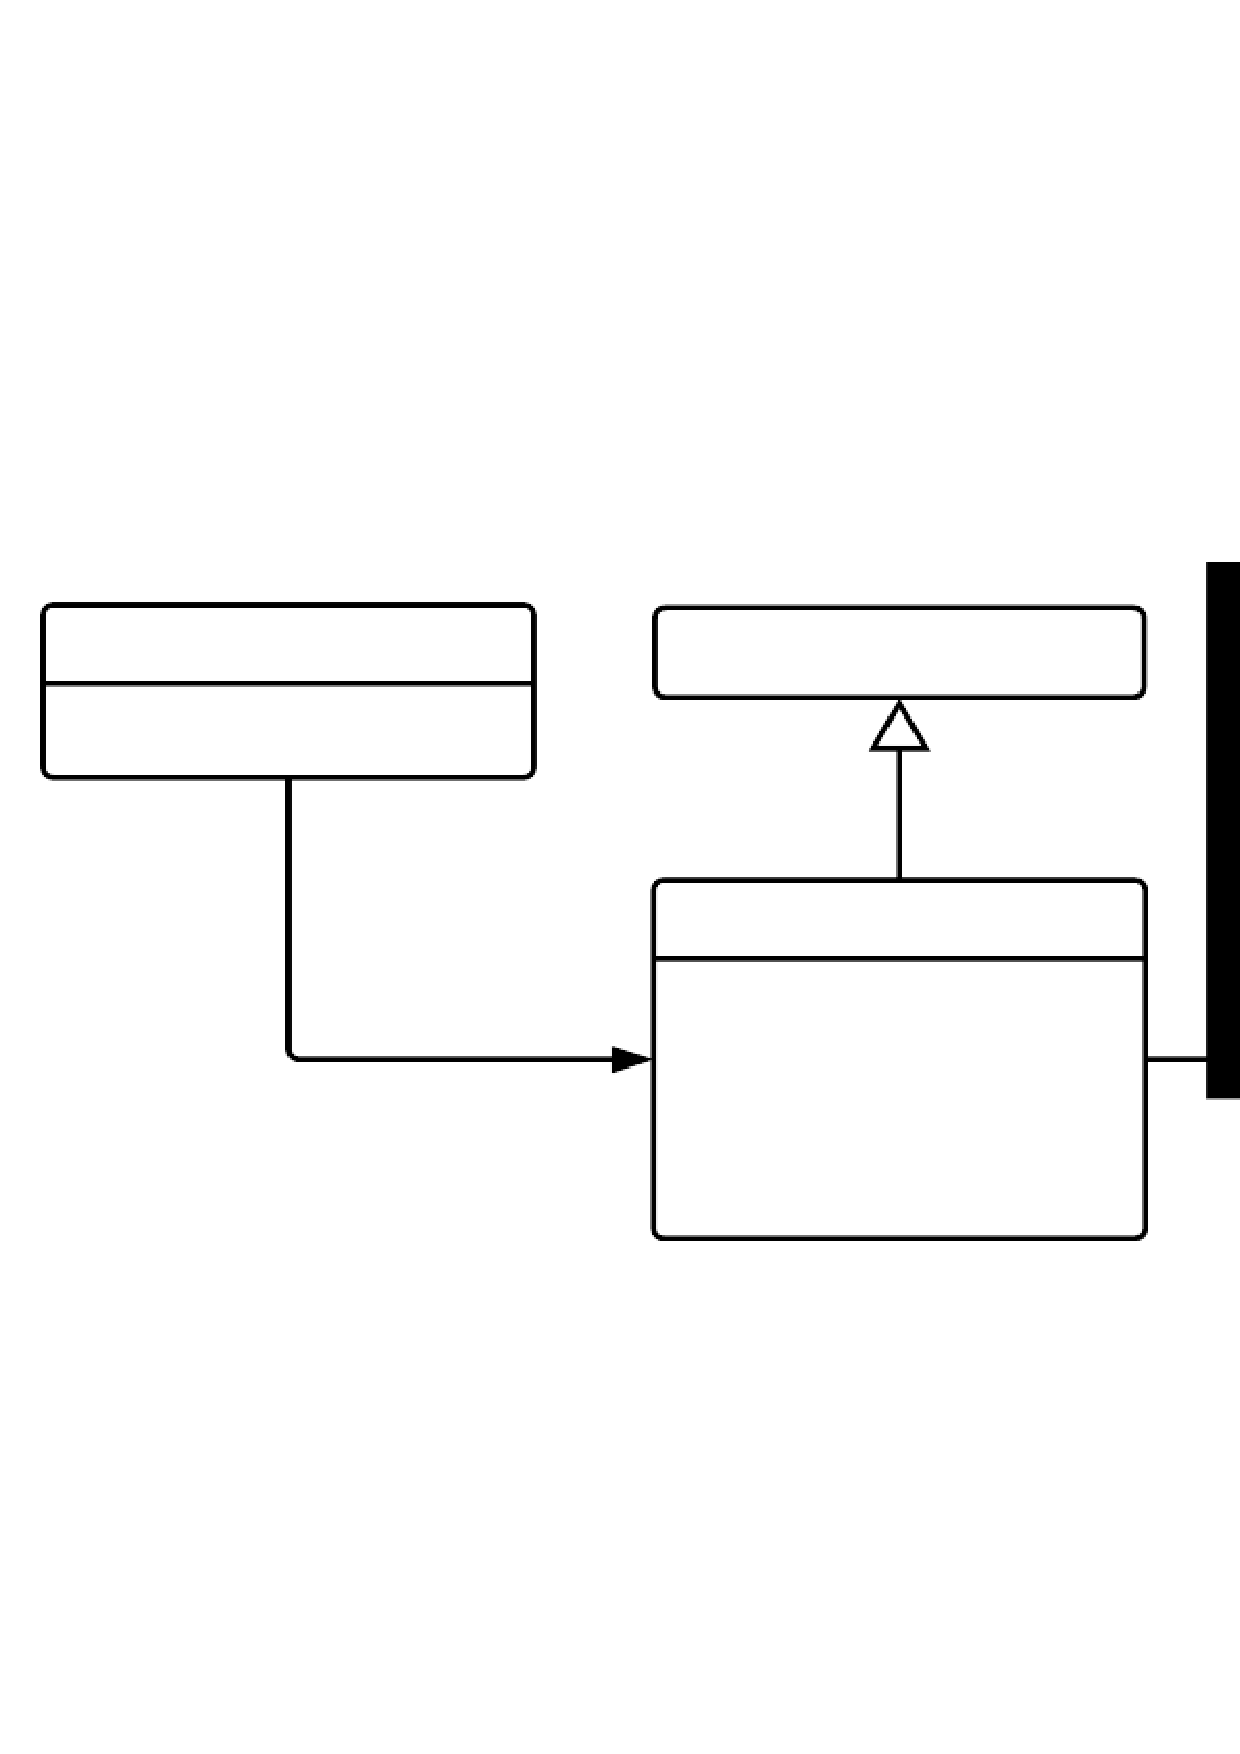
\includegraphics[width=1.0\textwidth]{logset-key-classes.png}
\caption{Key classes and predicates in the logset vocabulary. }
\label{f:logset-classes}
\end{figure*}

\begin{figure*}
\includegraphics[width=0.9\textwidth]{logset-classes-nodes.png}
\caption{Examples of some nodes and relationships published in different places 
from different sites (indicated via color), forming a single global graph. }
\label{f:logset-classes-nodes}
\end{figure*}

\begin{figure*}
\includegraphics[width=0.9\textwidth]{logset-example.png}
\caption{Key classes and predicates in the logset vocabulary. }
\label{f:logset-example}
\end{figure*}

\subsection{Annotation Schema}

The primary goal of annotation is to provide a reduced set of searchable,
understandable data that can hint at relationships between logged 
events and guide the user to further searches and to interesting locations
in the raw log data. Along with our identified requirements, this 
provides some design requirements for the schema:

\begin{figure}
\includegraphics[width=0.4\textwidth]{annotations.png}
\caption{Annotations provide reduced, tractable view of significant events
in a much larger volume of log data.}
\label{f:annotations}
\end{figure}

\begin{itemize}
\item Temporal and subject (system and component) information are 
      the key fields, along with a human readable description, the 
      annotation itself.
\item The raw logfiles that the annotation concerns should be identified,
      if possible.
\item Multiple people should be able to annotate the same underlying 
      log data, and users of the annotations should be able to 
      identify annotators to request more information, if necessary.  
\item The architectural relationships between components indicated in 
      annotations should be accessible, in order to facilitate 
      traversal from an annotation of interest to annotations relating to
      components that may have impacted it.
\item Annotation fields should support searching based on the subject type 
      of an annotated event (such as a network event) or other 
      related information.
\end{itemize}

\subsubsection{The schema}

%In this subsection we describe the major fields necessary to support the
%architectural requirements that pertain to the annotations themselves
%(as opposed to the remote discovery infrastructure). The prototype
%implementation is an SQLite database, so we descirbe in in terms
%of that implemention, however that is not required. More generally
%this would be descirbed in terms of accessor APIs independent of
%the implementation beneath them.
Our annotation schema is an SQL database definition with a central 
``annotations'' table:

\begin{figure}[H]
\begin{small}
\begin{minted}{sql}
CREATE TABLE 'annotations' (
       id             integer,
       authorid       char(3) NOT NULL,
       description    text NOT NULL,
       -- timespan of the action or event:
       starttime      datetime NOT NULL,
       endtime        datetime NOT NULL,
       -- impact of the action or event:
       startstate     text,
       endstate       text,
       systemdown     boolean,
       system         text,
       components     text,
       -- was the event manually induced?
       manual         boolean,
       -- subject type and annotation context:
       LDcategory     text,
       LDtag          text,
       balerpatternid integer,
       -- event source:
       logfiles       text,
       PRIMARY KEY('id','authorid')
        );
\end{minted}
\end{small}
\caption{The central annotations table definition. }
\label{f:ann-table}
\end{figure}

The id, source, description and temporal fields are self-explanatory. 
The impact fields are designed to aid exploratory analysis, for example
\texttt{startstate} and \texttt{endstate} can be used to indicate that
a component that was in a \texttt{faulty} was either \texttt{repaired}
or \texttt{flagged} by the end of the event. A \texttt{systemdown} flag
allows search for events resulting in a full system failure.

The \texttt{system} and \texttt{components} fields correspond to the 
\texttt{Subject} class of the RDF vocabulary.
For the Cray system we define \texttt{node}, \texttt{blade}, \texttt{chassis},
\texttt{cabinet}, \texttt{router}, \texttt{tile}, \texttt{link}, \texttt{nic},
\texttt{smw}, and \texttt{other}, all of which (except \texttt{other}) are 
also \texttt{SubjectType}s described in RDF in data dictionaries and can, in
combination with the \texttt{system}, identify a specific component.

The \texttt{components} may be identified with finer granularity than
is represented in the RDF graph - for example \texttt{c0-1c0s4n0}. One 
envisioned source of machine-generated annotations is LogDiver~\cite{LogDiver}, 
a tool developed by UIUC which associates regular expressions defining
events in log files of interest with categorizations including 
\texttt{node/blade},
\texttt{scheduler}, \texttt{storage}, \texttt{network}, \texttt{cooling/facilities/sensors},
\texttt{power}, \texttt{system software}, \texttt{datawarp}, and \texttt{unknown}.
These also correspond to \texttt{SubjectType}s in an RDF dictionary.

The \texttt{manual} flag indicates that an event was manually induced,
such as an administrator action to take down a node as opposed
to the system taking down a node because it failed a health check.
Knowledge of this can be used to more accurately determine the
number of true failure events and for assessing the effectiveness
and availability of system resilience mechanisms


% not sure ofthe context here... (other tables?):
%Note that event may have many relationships. We choose to limit them to one each to address
%the requirement of searchability. It is expected that exploration will facilitate dsicovery
%of events, even when the first order assocation may be off; also discovery of assocationed
%events in different subsytems can help understanding of how events propagate in a system.


\subsubsection{Other tables}

The schema includes some supporting tables:

\begin{description}
\item[Meta Annotations] \hfill

      The \texttt{metaannotations} table supports annotation sets,
      wherein a collection of annotations relates to a single larger
      event
      
\item[Component Aliases] \hfill

      Different components are identified differently in different log 
      series, for example the same node on a Cray XC might be called
      \texttt{nid00001} by the scheduling system, \texttt{c0-0c0s0n1}
      by the boot system and even its IP address by another log source.
      
      To support this we define an \texttt{aliases} table, mapping 
      equivalent component names. This is generally populated via
      \texttt{/etc/hosts}, or on Cray systems, the output from
      \texttt{rtr --system-map}
      
\item[Architectures] \hfill

      The topologies of current clusters are more complex than
      a simple hierarchy, so we support the definition of multiple
      architectures to describe relationships between components.
      We have defined three architectures for Cray systems, these
      are described below. 
      %in Section~\ref{s:hierarchies}.
      
\end{description}

\subsubsection{Component hierarchies}
\label{s:hierarchies}

We have identified three distinct architectures within a Cray cluster:

\begin{enumerate}
\item The \texttt{physical} architecture consists of parent-child or
container-contained associations, such as a \texttt{cabinet - chassis}, 
\texttt{blade - router}, \texttt{router - link} and \texttt{router - nic}.
This table is populated from the system definition - for example on a 
Cray XC each cabinet holds three chassis, so an entry might look like:

\begin{small}
\begin{verbatim}
id  type  cname  parent  children
1   CAB   c0-0   smw     c0-0c0,c0-0c1,c0-0c2
\end{verbatim}
\end{small}

The \texttt{physical} architecture supports discovery of faults 
propagating from child to parent components.

\item The \texttt{router} architecture describes network topology
from the perspective of the router - for example an Aries has 
(blue:black:green) links while a Gemini has X:Y:Z. This supports
discovery of event propagation across neighboring routers:

\begin{small}
\begin{verbatim}
id  type  cname        NICS [...]   nettopo
10  RTR   c0-0c0s10a0  c0-0cd0...   0:0:10
11  RTR   c0-0c0s11a0  c0-0c0s...   0:0:11
12  RTR   c0-0c1s0a0   c0-0c1s...   0:1:0
13  RTR   c0-0c1s1a0   c0-0c1s...   0:1:1
\end{verbatim}
\end{small}


\item The \texttt{link} architecture supports 
discovery of faults propagating across connected components,
such as a node failure disabling a link and contributing to 
congestion conditions on its peer node.

\begin{small}
\begin{verbatim}
id  type E0            E1            
16  GRE  c0-0c0s0a0l20 c0-0c0s4a0l22 
\end{verbatim}
\end{small}


supports determination if an event affects the
components at teh other end of a network link. The router architecutre
supports determination of proximity of events in the network topology.
We chose to separate architecutres in order to enable different
search and interpreation of events which affect components with
different \texttt{association} with each other. 
\texttt{associations}
include \texttt{parent-child: component-component} as opposed to
\texttt{parent-child: router tile}, or \texttt{peer: HSN link}
as opposed to \texttt{peer: Router-NIC} or \texttt{peer: NIC-Proc}.
To represent more globally associated, such as SMW
events which can directly affect all components, we define
a \texttt{supremum} relationship.

\end{enumerate}


To support discovery of events propagating over connected or related 
components our schema includes Architecture tables

At the resolution of log entries 

\texttt{Components} can include the compute and any supporting subsystems,
such as storage and facilities related elements. For the Cray system
itself, we define \texttt{node}, \texttt{blade}, \texttt{chassis},
\texttt{cabinet}, \texttt{router}, \texttt{tile}, \texttt{link}, \texttt{nic},
\texttt{smw}, and \texttt{other}.

In order to enable dsicovery of events which are either reported on related
compoentns or that propagate amont components we support the defintion
of \texttt{architectures}. For the Cray system itself, we define three.







In the prototype, we define all architectures and relationships,
however we currently prinipally search the physical topology only
and support recursive search up and down, including for supremum
relationships. We are working on tools to better enable search of
the multiple architecture represenations.

In order to determine the effect of events on jobs, we also
intend that job data be made availble with the annotations.
We expect only the current common fields (e.g., starttime,
endtime, components, etc) exposed in scheulder logs or
interfaces.








\subsection{Tools}

There is no technical issue preventing someone from cataloging, 
annotating and investigating a dataset 
by manually writing RDF files, populating an annotation database 
and running SQL and SPARQL queries against them. However, 
the schema and vocabulary are accessible to a much wider 
audience with the aid of tools that ease the learning curve and automate many of the processes.

In the course of this work we have developed a small collection 
of tools for constructing and querying graphs and annotation databases.

%\begin{itemize}
%\item get.py for querying an annotation database
%\item what do we have for building an annotation database? (Ann's tool for %ingesting the mutrino and jobs info?)
%\item framework for working with rdf graph
%
%(plan is to have cataloging and running general queries supported at least, and ideally also slicing-and-fetching of timestamped logs in line-per-timestamp format)
%\end{itemize}

\subsubsection{Cataloging log sources and archives}

For easier use of the RDF graph we have developed a framework, in 
the form of a python package \textcolor{red}{cite github address?}
for constructing and querying the graph. The package is still pre-release
and in active development; so far, its capability is limited to 
walking a directory tree to discover and catalog log files --with 
some constraints on the types of log files it can inspect-- and some 
basic querying. The design is extensible: a small interface
is defined for handlers of file and log format types and additional 
handlers can be easily added to the toolkit.

Much information must be collected to create useful metadata: most of
this can be automatically inferred by querying the graph and inspecting 
the file (for example, the filename hints at the likely \texttt{LogSeries},
temporal boundaries can be discovered by reading the first and last records
and the subjects for a tree of log data can be inferred from a coarse-grained subject (such as the cluster) and information held by each \texttt{LogSeries}. Details requiring human input are acquired through 
a simple question-and-answer interface that presents the user with 
reasonable guesses and prompts editing and confirmation. In this manner 
thousands of logs can be described based on only a handful of user 
interactions.


\subsubsection{Querying Annotations}
\label{s:querying}
A stated goal of our project is to enable annotation of log data so that researchers can analyze it with sufficienct context to understand what was happening on the system when a given set of loglines were written. However, such a tool would also enable consultants and users to make sense of log data in order to better address questions about job failures. Neither use case would be addressed, however, without an efficient means of querying the annotations. We have therefore created a python-based query engine for that purpose.

The query engine offers a set of command-line flags to customize a query. Users can combine them for highly specific queries without resorting to complex SQL. A user can refine a query by start (-s or --start) and/or end (-e or --end) time, by component name (e.g., node or slot cname, -c or --component), by type (descriptive phrase, such as "link down", -t or --type), or by any of the columns in the database schema (-t columnname=foo). In addition, a user can specify a job ID (-j or --job) to retrieve annotations on logs written during the time of the job and affecting any of the nodes on which it ran. Adding the -a or --after flag enables the user to specify a complex query with a single timestamp and retrieve the next single instance of a match for the query.

In addition to specifying a single component, a user can retrieve annotations for related components, traversing the architecture of the system to a specified depth (-d or --depth), or number of hops. For example, a query for a component specified to depth 2 would retrieve parent and grandparent components as well as child and grandchild components. 
For any depth search, any supremum (eg SMW) or `unknown' components are also queried.
This flag leverages a table of physical components in the database that reflects the architecture of the system for which the annotations were made. 

The user also has options for viewing the retrieved annotations. Formatting options include a table (-f table), a JSON array (-f json), or the default textual listing Figure~\ref{f:default_format}. The user may choose to increase verbosity (-v, -vv) or to limit the maximum number of retrieved annotations (--limit).

An additional query for jobs (--jobs) allows the user to enter one or more annotation identifiers and retrieve the list of job IDs that could be affected by the annotation, based on the time and the nodes on which they ran.

The current query engine retrieves annotations only, though the annotation metadata provides sufficient information to locate relevant log files. We plan to enable retrieval of subsets of the logs through the tool in the future.

\begin{figure}
\begin{small}
\begin{minted}{sql}
----------
[822659] by acg on system Mutrino
Time: 2015-04-29 18:16:32 to 2015-04-29 18:16:32
Start state: None ; End state: None
Description: Correctable memory error. This may result in degraded performance.
Manually invoked? False ; System down?:  False
Components: ["c0-0c1s8a0n0"]
Tags:
LogDiver category group: NO
Baler pattern ID: 280
Relevant log files: hwerrlog
----------
[822660] by acg on system Mutrino
Time: 2015-04-29 18:16:42 to 2015-04-29 18:16:42
Start state: None ; End state: None
Description: Correctable memory error. This may result in degraded performance.
Manually invoked? False ; System down?:  False
Components: ["c0-0c1s8a0n0"]
Tags:
LogDiver category group: NO
Baler pattern ID: 280
Relevant log files: hwerrlog
----------
[822661] by acg on system Mutrino
Time: 2015-04-29 18:16:52 to 2015-04-29 18:16:52
Start state: None ; End state: None
Description: Correctable memory error. This may result in degraded performance.
Manually invoked? False ; System down?:  False
Components: ["c0-0c1s8a0n0"]
Tags:
LogDiver category group: NO
Baler pattern ID: 280
Relevant log files: hwerrlog
*** Done! ***

\end{minted}
\end{small}
\caption{Annotations as returned by the query engine in default format. }
\label{f:default_format}
\end{figure}


\subsubsection{Creating Annotations}


Annotations can be added to a database by several means. The simplest approach would be with an SQL insert at an sqlite command line, but this method can be tedious and relies on manual input. One simple way of adding a large batch of annotations is to enter them as a spreadsheet in CSV format, using a small uploader script which we provide. These approaches work well for human-generated annotations, such as individual observations from a system administrator or output from a ticketing system.

To faciliate the automated creation of log line annotations
and the identification of the occurrences of events to be annotated,
we have been using two external tools, Baler and LogDiver (described in more detail below).
In support of these we have developed tools to create annotation using output from these.

Note that a single or even multiple SQL databases are not required by our design. A plugin interface to a component presenting an API which could return similar annotation information would also be appropriate (e.g., one could front a tool with its own datastore). However, to enable a simple, consistent format for portable general release of an annotated dataset we do so, as described in the next section.

\section{Proof of Concept}
\label{s:proof}
To faciliate the creation of log line annotations
and the identification of the occurrences of events to be annotated,
we have been using two tools.

LogDiver~\cite{LogDiver} is a tool developed by UIUC which includes a set of regular expressions defining
events in log files of interest; the regular expressions are associated with categorizations
which are a subset of those described in the previous section; the
category name, \texttt{LDcategory}, was chosen to reflect our intention to map to the
LogDiver categorizations where possible.
LogDiver itself is used to discover the occurrences of the regular
expresssions in the logs and to determine statistics and information about event sequences
such as statistics of failure events, or of timings of failures and recoveries.
LogDiver, or any such regex-based tool (e.g., SEC~\cite{SEC}), can be used to efficiently extract events
for subsequent annotation, based on the intention for the existence of the regex.

For the dataset described in this work, we prinicpally used Baler~\cite{Baler} for
identifying the log lines to be annotated and for extracing them from the dataset.
Baler extracts patterns from log files without requiring apriori knowledge of
regex of interest. Rather, Baler takes dictionaries of ''words''; words appearing in the log lines
are the passed through to the pattern and non-words become a wildcard in the pattern.
Wildcards of certain formats, for example numbers, hex dumps, char arrays, hostnames and link names
(in cname format for Cray systems) are represented as that formatted type in the pattern.
For example, every instance of the log message \texttt{mutrino-smw 24626 found\_critical\_aries\_error: Processing ''PCI-e CMPL\_TIMEOUT'' critical error (0x660e)}
is represented by the pattern \texttt{<host> nlrd <pid> found\_critical\_aries\_error: Processing ''* *\_TIMEOUT'' critical error (<num>)}.
This illustrates where words, formatted wildcards, and unformatted wildcards (represented by \texttt{*}) appear in the pattern.

For Cray systems, we augment
the dictionary with an architecture specific dictionary of about 100 words (e.g., Lustre, DIMM).
For 3 months of data from our Trinity test system, Mutrino, a 100 node XC 40,
we had over 120 million text log lines which were reduced to 15,500 patterns. To further identify patterns
of interest, we weight the patterns by the occurence of 50 weighted
keywords (e.g., congestion = 1.5, error = 1.5, degrade = 0.75). This further reduced the patterns
to 2,500 significantly weighted patterns. For example the pattern
\texttt{<host> nlrd <pid> ***ERROR***: Link recovery operation failed; error <num>} has
an aggregate weight of 5.5. From those, we chose 150
patterns to annotate with enhanced descriptions. This resulted in about 860,000
annotated log line instances.

It is our intention to
build a plugin to interface with Baler, and support the annotations there,
however in the prototype, we merely annotated the extracted patterns from
Baler and loaded them into a single database.
We include the Baler pattern id in the annotation fields
for reference ease; only the annotation description, not the original log line nor the pattern
are stored in the annotation database.

Some example patterns, from which the originating log line will be obvious, and
the resulting annotations used in this work, are given in Figure~\ref{f:baler}.

\begin{figure*}
\begin{annol}

Baler pattern, preceeded by weight (W=#) and balerpatternid number:
(W=5)        258   HWERR[<host>][<num>]:<num>:SSID RSP A_STATUS_ORB_TIMEOUT Error:*=<num>:*=<num>:*=<num>
Annotation:
authorid:acg  description: 'ORB timeout waiting on outstanding request(s) in the buffer'  LDcatgroup: NE

Baler pattern and weight:
(W=3.75)     498   <host> nlrd <pid> do_set_alerts: <num> links failed, <num> blades failed, <num> blade critical faults, *_in_progress <num>, *_*_reroute <num>; reroute required
Annotation:
authorid:acg  description: 'Setting alerts due to failures. A network reroute is required' LDcatgroup: NE

Baler pattern and weight:
(W=3.25)     748   <host> nlrd <pid> ***ERROR***: Warm swap operation failed; error <num>
Annotation:
authorid:acg description: 'Warm swap failed. This is in response to a operation intended to reset/reinit/replace a component (including network components).' LDcatgroup: NO

Baler pattern and weight:
(W=1.5)      705   <host> nlrd <pid> responder_work_*: Top <num> nodes involved with network congestion
Annotation:
authorid:acg description 'System computing and listing congestion candidate applications' LDcatgroup:NE
\end{annol}
\caption{Example Baler patterns extracted from log lines and their annotated versions. Events to annotate are based on
knowledge of significant events. Annotation descriptions can provide additional context to non-self-explanatory log messages.}
\label{f:baler}
\end{figure*}


We fed Baler with the Cray logs in the format in which they reside on the smw. This required us
to do some file-specific format extraction of messages, timestamps,
and components (e.g., \texttt{netwatch}, \texttt{hwerrlog}) which we may not have had to do if
we had fed it raw syslog versions of the files or datastream; however, this also enabled us
to include the log file type (e.g., \texttt{nlrd}, \texttt{hwerrlog}) in the pattern metadata,
which aids the log file look-up. 

For many cases, messages are reported
on the smw with the component association of the smw. For some cases, we can
extract the actual component of interest. For example, from the Baler pattern
\texttt{<host> nlrd <pid> found\_critical\_aries\_error: handling failed * link on <host> (node )}
we can infer the fields from which to extract the \texttt{host} and \texttt{node} to which
the annotation should be associated. Other messages refer to actions by the SMW for which
the component cannot be inferred. In these cases the component assignment will either be
the smw or 'unknown'.

We used Baler for all major log processing, except for the \texttt{command} log, which required us
to associate \texttt{START} and \texttt{END} of events, for which we used a perl script. This
log includes both manually initiated and automatically invoked commands of
interest such as warmswaps, boots, etc. This was particularly useful for
determining manual actions that may not have been well documented by the
system administrators. This resulted in another 2,000 annotations. In addition,
we extracted the times of reboots from the datetime in the name of the \texttt{p0-XXX}
directories. All annotations from these two sources are attributed as manually induced.

Some other system administrator actions were recorded by manually generated annotations
(about 10, in this case). Ticketing systems may be used to generate such annotations as well.
Knowledge of such events is useful for understanding the root causes and resolution of errors
in the dataset. These annotations were generated manually.

Other non-log events include external actions by non-administrators
such as facilities tests, fault injection research, which require
annotations by differnet people. These were also generated manually
for this dataset. Similar to the Baler Annotations, for the
prototype these were loaded into the same annotation database.

Log data was extracted from alps logs, which was the scheduler in use for
this time period. This could be replaced with queries to a slurm,
or similar, database or interface, where available.

Recall that the main aim of the annotations
is to provide a reduced set of searchable, understandable data, with the
ability to use the annotations to further more detailed search of the raw
logs, if possible and desired. This differs from tools
such as SEC, which is intended to enable action upon the run time
occurence of a log line matching a regex (e.g., notification
of failed component), or Splunk, which is intended
to facilitate knowledge of the occurences of pre-defined
events with accompaning statistical plots.

















